\documentclass[aps,prl,twocolumn,superscriptaddress,nofootinbib]{revtex4-1}

% the percent sign gives comments in Latex
% top line indicates this is for Physical Review, standard journal format,
% suitable for electronic submission of articles

% the line above is necessary to start any latex document.
% this is one variation that should work for most things.
% if you want double spaceing, use the following:
%
%\documentclass[prd,preprint,letterpaper]{revtex4}
%
% the "preprint" designation will make a wider line
% spacing, good for markup.
\usepackage{graphicx}  % this is the up-to-date package for all figures
\usepackage{amssymb}   % for math
\usepackage{verbatim}  % for the comment environment
\usepackage{color}
\usepackage{gensymb}
\usepackage{amsmath}

\usepackage[section]{placeins}

\usepackage{wrapfig}
\usepackage{hyperref}
\usepackage{titlesec}
\usepackage{amssymb}   % for math
\usepackage{verbatim}  % for the comment environment
\usepackage{color}
\usepackage[nodisplayskipstretch]{setspace}
\usepackage{amsmath}
\usepackage{blindtext}
%\usepackage[pdftex]{graphicx}
\usepackage[outdir=./]{epstopdf}
\usepackage[space]{grffile}
\usepackage{epsfig}
\usepackage[separate-uncertainty=true]{siunitx}
\usepackage{tikz}
\usepackage{pgfgantt}
\usepackage[english]{babel}
\usepackage[utf8]{inputenc}

\titlespacing*{\section}
{0pt}{1\baselineskip}{.5\baselineskip}

\titlespacing*{\subsection}
{0pt}{.5\baselineskip}{.3\baselineskip}

\usepackage{footnote}

\bibliographystyle{apsrev}


% these are some custom control of the page size and margins
% \topmargin= 0.2in  % these 1st two may be needed for some computers
% \textheight=8.75in
%\textwidth=6.5in
%\oddsidemargin=0cm
%\evensidemargin=0cm

% this is where the actual document itself (rather than control statements) begins:

\begin{document}

% use a style that gives automatic headings
%\pagestyle{headings}



% the \title{} command generates a title.

% the \\ below is used to FORCE a line break in the middle of the sentence--
% otherwise latex computes it for you

\title{The Speed of Light}


\author{\textbf{Bryan Yamashiro}}
\author{Christina Nelson}
\author{Corey Mutnik}
\author{Daichi Hiramatsu}

\affiliation{Department of Physics \& Astronomy, \\
University of Hawaii at Manoa,\\
2505 Correa Rd, Honolulu, HI, 96822, USA}





	      % \section is used to start a new one with a heading
\begin{abstract}

We measured the speed of light in an experimental apparatus against the constant value,\,\textit{c}, 299,792,458\,m/s. Instruments used to measure the speed of light included a light emitting diode\,(LED), a photomultiplier tube\,(PMT), and fast pulse circuitry. Measured speeds of light using leading edge linear fits were (3.06$\pm$0.16)$\times$10$^8$\,m/s and (3.13$\pm$0.50)$\times$10$^8$\,m/s for the applied pulse widths of 2\,ns and 40\,ns. Conversely, using asymmetric Gaussian fits, the speed of light measurements were (3.01$\pm$0.04)$\times$10$^8$ for 2\,ns and (2.97$\pm$0.02)$\times$10$^8$ for 40\,ns.




\end{abstract}

\maketitle    % this line is necessary to tell latex you are done with all
	      % of the stuff associated with the title, and now it can go
              % ahead and generate the title portion


\section{Background}

The method of measuring the speed of light used in this study is modeled after the Foucault method, which used an apparatus containing sets of mirrors to project and measure light. The projected light reflects off a rotating mirror, to a fixed mirror, back to the rotating mirror, finally to a detector. The apparatus was optimized by Albert Michelson in the 1920's and experimentally measured the speed of light to an error of $\pm$4\,km/s\,\cite{1}. Apparatuses such as the Foucault apparatus allow for measuring the speed of light in a laboratory.

 % the ~\cite{ } is how you link a reference in the text. The references
 % themselves are at the end.

% one or more lines of space between paragraphs determines them

\section{Apparatus}



The experimental apparatus replicates the Foucault instrument, but without the rotating reflector. Values of the speed of light were measured with different applied pulse widths. Components include the time-to-amplitude converter\,(TAC), Multi-Channel Analyzer\,(MCA), and the computer program\,(MAESTRO)\,\cite{2}. It is important to note that the medium inside of the enclosed tube is air rather than a vacuum. As the name suggests, the TAC converts the pulse time into positive amplitude pulses whose pulse height is proportional to the time difference between the start time\,(t$_{start}$) and stop time\,(t$_{stop}$). Concurrently with the positive amplitude pulses, negative amplitude pulses are sent directly to the TAC, generating t$_{start}$. Photons emitted from the LED source travel the length of the tube and are transmitted to the PMT, which are then converted to t$_{stop}$ in the TAC. Photons from a second source are collected from reflections off the Fresnel lens. Both reflection phenomena generate two peaks, one with a relatively lower count rate in the respective amplitude bins. The MCA records the TAC signals and distinguishes the counts across 2048 channels. MAESTRO compiles all amplitudes with corresponding channels and generates histograms, also providing ASCII data. Components of the instrument are specified in figure 1.

\begin{figure}[h!]
  \begin{center}
\centerline{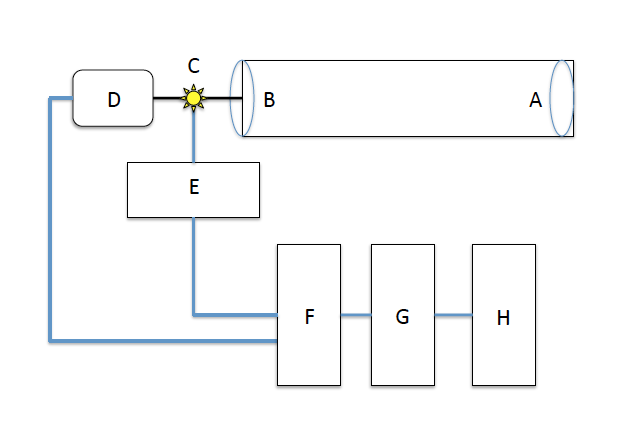
\includegraphics[width=3.in]{solapp.png}}
\caption{\it \small{A)\,Mirror, B)\,Fresnel lens, C)\,LED Source, D)\,PMT, E)\,Pulser, F)\,TAC, G)\,MCA, H)\,MAESTRO.\,\cite{3}. \label{fig1}}}
  \end{center}
\end{figure}

\section{Procedure}


\begin{table}[htb!] 
\caption{\it Initial Apparatus Parameters}
		%table caption at the top is standard
\label{t1}   % labels are used to refer to this in the text
 \begin{center}   % center the table on the page
    \begin{tabular}{|c|c|c|} \hline   % tabular environment determines the

Applied Pulse & Tube & MCA \\
Widths to LED & Length & Channels  \\
(ns)  & (m) & (sec.)   \\ \hline \hline
    % the "~" character forces a non-breaking space--here is just makes the columns a bit wider
4 \& 20 & 11.3183$\pm$0.0013 & 2048 \\ \hline
%20 & 445.6$\pm$0.05  &  2048  \\ \hline

     \end{tabular}
  \end{center}
\end{table}

% you always need to end an environment { } you have started--just like in C

The experiment uses a yellow LED emitting photons into the an enclosed tube\,\cite{3}. Emitted photons initially traveled through a Fresnel lens located in the enclosed tube, which also reflected photons. These photons were detected first by the PMT at an earlier time, $t_1$. Photons that were not backscattered pass through the Fresnel lens and were reflected off the mirror, A\footnote[1]{Corresponds to labels\,(A-H) in Figure 1}, on the back of the enclosed tube. The reflected photons were then detected at a delayed time, $t_2$. Photons were then converted into electrons via the photoelectric effect. Ultimately the pulses and the electrons were then converted into amplitude using the TAC and then split over multiple channels in a histogram compiled with MAESTRO.

\begin{figure}[h!]
  \begin{center}
\centerline{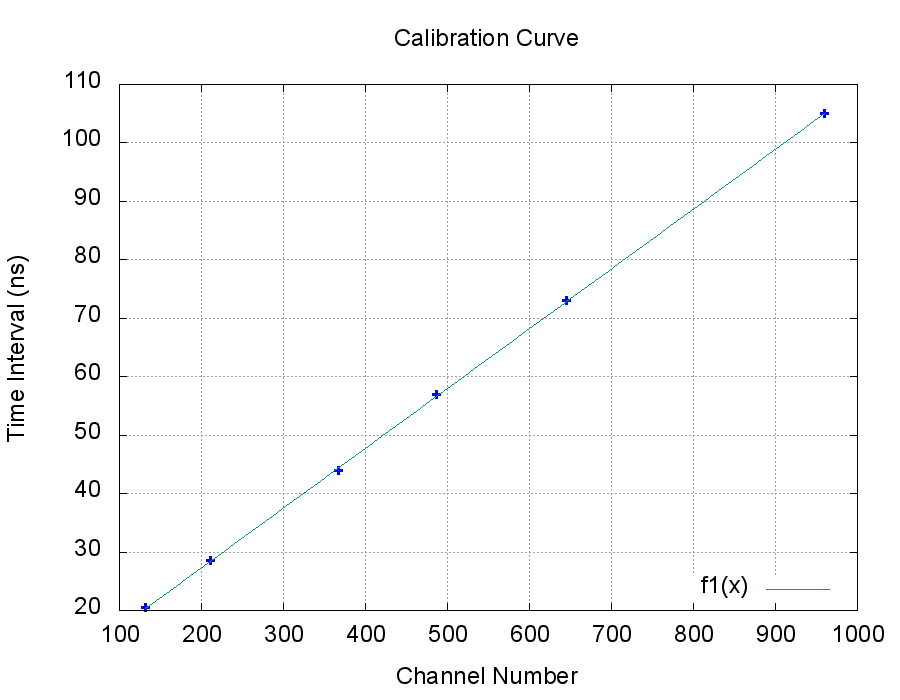
\includegraphics[width=3.5in]{calib.png}}
\caption{\it \small{A calibration curve for the TAC. The linear fit represents a correlation calibration between channel number and time. \label{fig1}}}
  \end{center}
\end{figure}

Using the delay box, a calibration curve was compiled to represent the time interval\,($\Delta$t) versus the MCA channel number for six unique time intervals. A linear fit of the six time intervals were used to convert the channel numbers for the difference in time between the histogram peaks generated by MAESTRO. Resulting time for the peak difference was utilized along with the measured enclosed tube length to determine an experimental estimate of the speed of light.
\\
\indent Two trials of different pulse widths were conducted for 2\,ns and 40\,ns. Nothing except the pulse widths were manipulated during this study to represent a fixed system with one changing parameter.





\section{Calculation of Results and Errors}

\begin{equation}
c = \frac{2L}{\Delta t}
\end{equation}

The measured speed of light, $c$, was calculated using equation 1. The variable, $L$, in the same equation represents the distance from the Fresnel lens to the mirror. Input parameters are shown in table 1. MAESTRO provided an ASCII data file resulting in figures 3 to 6. The set of figures show two peaks for both the 2\,ns and 40\,ns applied pulse settings.
\vfill\eject

\begin{figure}[h!]
  \begin{center}
\centerline{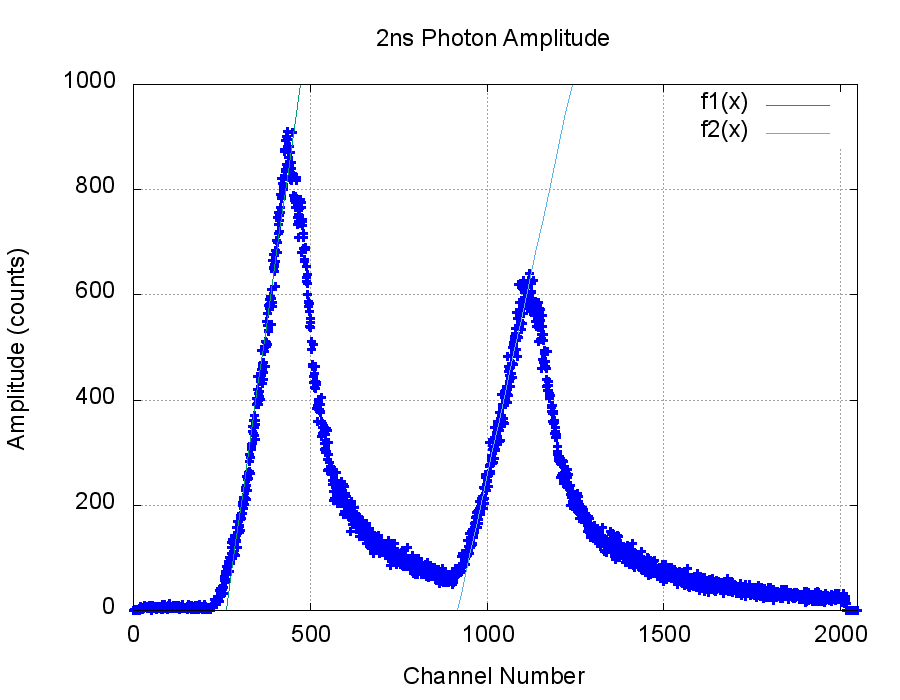
\includegraphics[width=3.5in]{solgraph2.png}}
\caption{\it \small{MCA channel distributions for a 2\,ns LED pulse setting with two leading edge linear fits. \label{fig1}}}
  \end{center}
\end{figure}

\begin{figure}[h!]
  \begin{center}
\centerline{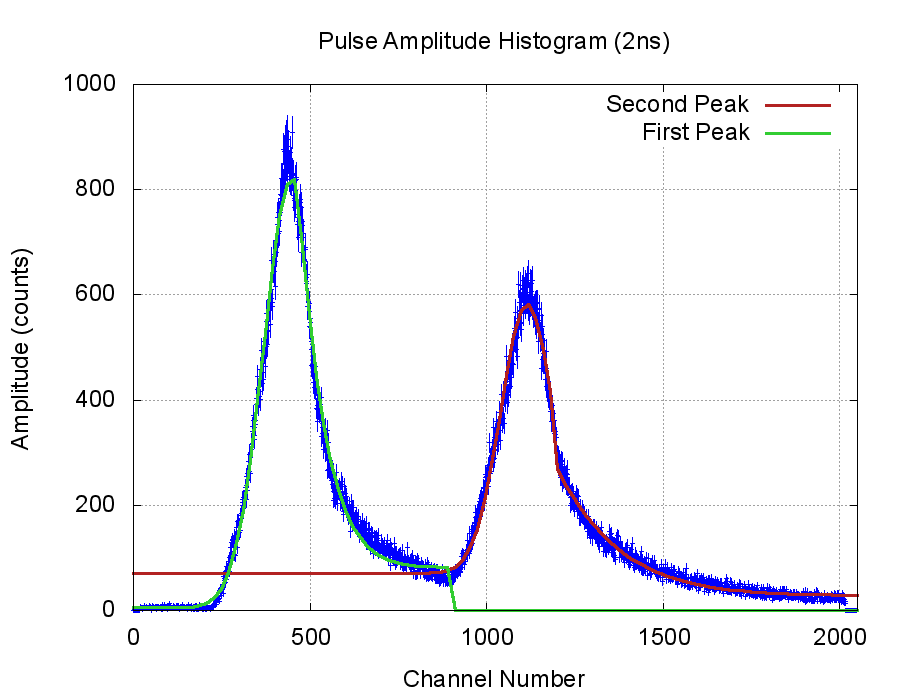
\includegraphics[width=3.5in]{2nsgauss.png}}
\caption{\it \small{MCA channel distributions for a 2\,ns LED pulse setting with asymmetric Gaussian fits. \label{fig1}}}
  \end{center}
\end{figure}


The two peaks correlate to the time of initial detection of reflected photons off the Fresnel lens, and the final detection of photons from the mirror at the back of the tube. Linear regressions were fit to the ascending slopes of the two peaks. The variance between the linear fits provided the difference in channel numbers for the two-photon detection phenomena. The channel difference was calibrated with the calibration curve to output a time difference, $\Delta$t. Using the initial length of the tube and time differences resulted in a measured speed of light using equation 1.

\begin{figure}[h!]
  \begin{center}
\centerline{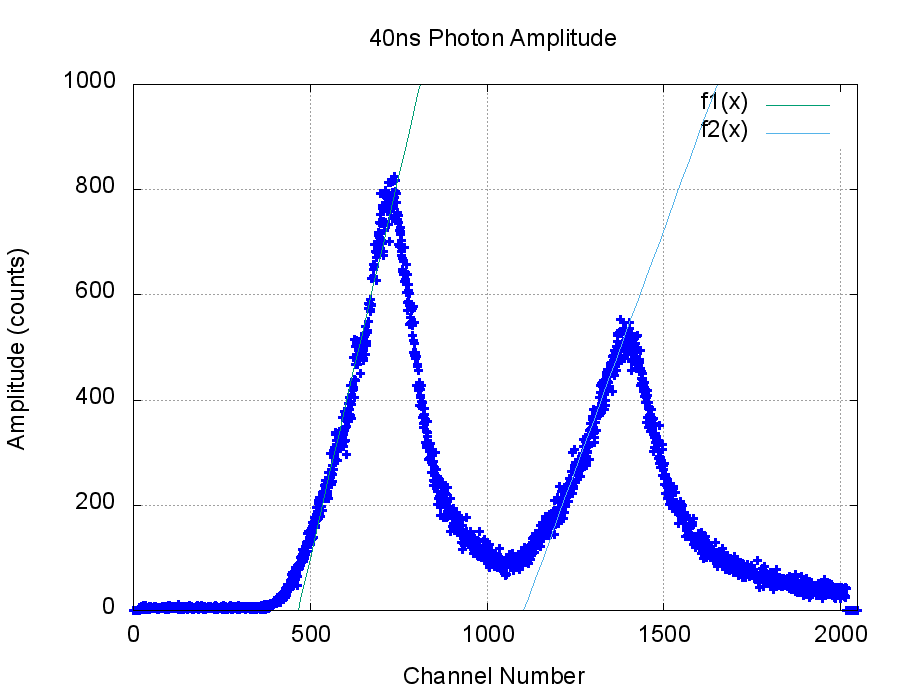
\includegraphics[width=3.5in]{solgraph40.png}}
\caption{\it \small{MCA channel distributions for a 40\,ns LED pulse setting with two leading edge linear fits. \label{fig1}}}
  \end{center}
\end{figure}

\begin{figure}[h!]
  \begin{center}
\centerline{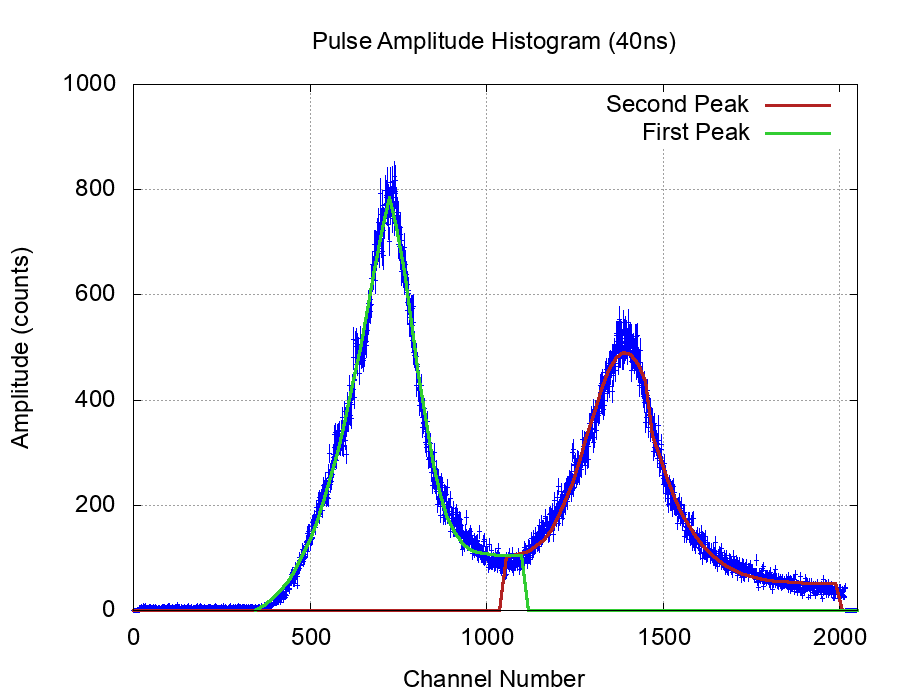
\includegraphics[width=3.5in]{40nsgauss.png}}
\caption{\it \small{MCA channel distributions for a 40\,ns LED pulse setting with asymmetric Gaussian fits. \label{fig1}}}
  \end{center}
\end{figure}

\vfill\eject

\subsection{Experimental Values of the Speed of Light}

The experimental speed of light measurements using the leading edge linear fits were (3.06$\pm$0.16)$\times$10$^8$\,m/s and (3.13$\pm$0.50)$\times$10$^8$\,m/s for the 2\,ns and 40\,ns respectively. Additionally, using asymmetric Gaussian fits generated speed of light measurements of (3.01$\pm$0.40)$\times$10$^8$ and (2.97$\pm$0.18)$\times$10$^8$, again for 2\,ns and 40\,ns respectively. 

\begin{table}[h!] 
\caption{\it Values of $c$ with linear and Gaussian fits}
    %table caption at the top is standard
\label{t1}   % labels are used to refer to this in the text
 \begin{center}   % center the table on the page
    \begin{tabular}{|c|c|c|c|} \hline   % tabular environment determines the

Applied Pulse & Fit & Speed of & Percent \\
Width to LED & Type & Light & Error \\
(ns)  &  & (m/s) &  (\%)  \\ \hline \hline \hline
2 & Linear & (3.06$\pm$0.16)$\times$10$^8$ & 2.11 \\ \hline
40 & Linear  & (3.13$\pm$0.50)$\times$10$^8$ & 4.54 \\ \hline \hline
2 & Guassian & \textbf{(3.01$\pm$0.04)$\times$10$^8$}& \textbf{0.31} \\ \hline
40 & Gaussian  & \textbf{(2.97$\pm$0.02)$\times$10$^8$} & \textbf{1.06} \\ \hline
%20 & 445.6$\pm$0.05  &  2048  \\ \hline

     \end{tabular}
  \end{center}
\end{table}

\vfill\eject
\indent The main source of error is attributed to systematic error. The data consists of many points with corresponding errors in amplitude; therefore the systematic error was determined with Poisson error. The employed method consisted of measuring the width of the data points before the peak. The width included points which enclosed the data and represented systematic error.


\begin{savenotes}
\begin{table}[h!] 
\caption{\it GNUplot generated errors for 2\,ns applied pulse widths for both fits}
    %table caption at the top is standard
\label{t1}   % labels are used to refer to this in the text
 \begin{center}   % center the table on the page
    \begin{tabular}{|c|c|c|} \hline   % tabular environment determines the

          & First Peak  & Second Peak        \\ \hline
Slope\footnote{Leading edge linear fit}    & 4.77$\pm$0.05  & 3.09$\pm$0.04      \\ \hline
y-intercept\textsuperscript{a} & -1252.70$\pm$18.88 &   -2839.74$\pm$42.42  \\ \hline
Channel Numbers\footnote[2]{Asymmetric Gaussian fit}   & 448.46$\pm$8.91   & 1116.82$\pm$0.7754       \\ \hline


%20 & 445.6$\pm$0.05  &  2048  \\ \hline

     \end{tabular}
  \end{center}
\end{table}
\end{savenotes}

\indent Complete error propagation included the channel number difference of the linear and Gaussian fits and the calibration curve, also including the Poisson systematic error. Raw data from the fitting program yielded values and corresponding uncertainties shown in table 3. Compared to the true speed of light, $c$, the experimental speeds are within the experimental error, with the favored method being asymmetric Gaussian fits.


\section{Discussion}

Measured speeds of light were determined to be similar to the theoretical speed of light. The double linear fits provided channel differences leading to a stable estimate of the time difference. Asymmetric Gaussian fits were significantly more accurate for the applied pulse widths, relative to the leading edge linear fits, bringing percent errors below 2\%. Length of the tube was affected by extra slack in the measuring tape. In conclusion, the measurements of speed of light deviated from the accepted value of, $c$, but the experimental values are well within the systematic uncertainty.


% the following \setlength is to force the bibliography to have no
% paragraph indentations.Can use vairous units--cm are used here.
\setlength{\parindent}{0cm}

\begin{thebibliography}{99}  % the trailing 99 controls some obscure format--just use

\bibitem{1} McFarland, Kevin. "Speed of Light Demonstration by the Foucault Method." University of Rochester. Web. 5 Nov. 2015.     % {\em } for emphasis, \textbf{ } for boldface

\bibitem{2} "Multichannel Analyzer (MCA) Application Software." Nuclear Applications Software|ORTEC Scientific Equipment. ORTEC. Web. 5 Nov. 2015.

\bibitem{3} THE SPEED OF LIGHT. (n.d.). Retrieved November 4, 2015, from \url{http://www.phys.hawaii.edu/~teb/phys480l/SpeedOfLight.txt}




\end{thebibliography}





\end{document}

